\documentclass[titlepage, letterpaper, 10.5pt]{article}
\usepackage[letterpaper, margin=1.25in]{geometry}
\usepackage{graphicx}
\usepackage{comment}
\usepackage{amsmath}
\usepackage{caption}
\usepackage{subcaption}
\usepackage{nicefrac}
\usepackage{verbatim}
\usepackage{tablefootnote}

\begin{document}

\title{Phase Locked Loop}
\author{Ben Lorenzetti}
\date{Start Date: April 2, 2015\\
Submission Date: April 20, 2015}
\maketitle

\clearpage
\mbox{}
\thispagestyle{empty}
\clearpage
\setcounter{page}{1}

\tableofcontents

\section{Objective}

To measure the characteristics of a phase locked loop and to investigate and model its behavior in an FSK (frequency-shift keying) demodulator.

\clearpage
\section{Principles of Operation}
\label{principles-of-operation}

\begin{figure}[ht]
	\centering
	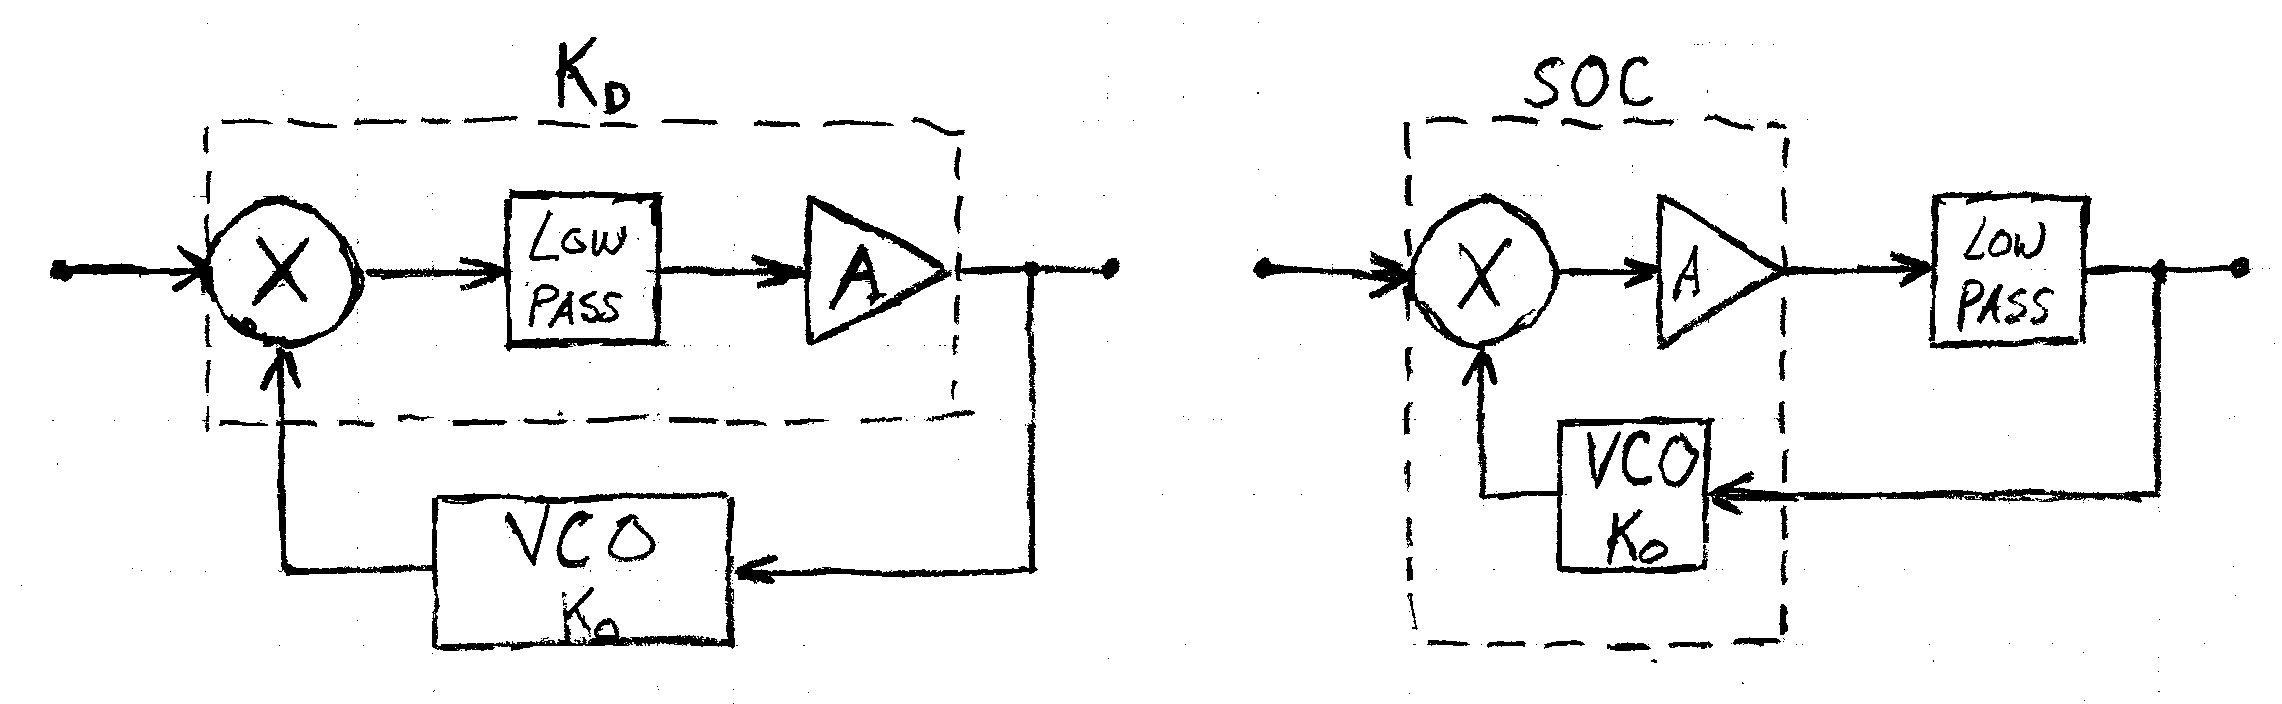
\includegraphics[width=0.7\textwidth]{diagrams/pll-demodulator-block-diagram}
	\caption{PLL Demodulator Block Diagram (left); Rearrangement for SOC Integration (right).}
	\label{pll-demodulator-block-diagram}
\end{figure}

\clearpage
\section{Theory}

\subsection{Texas Instruments LM656}

\begin{figure}[ht]
	\centering
	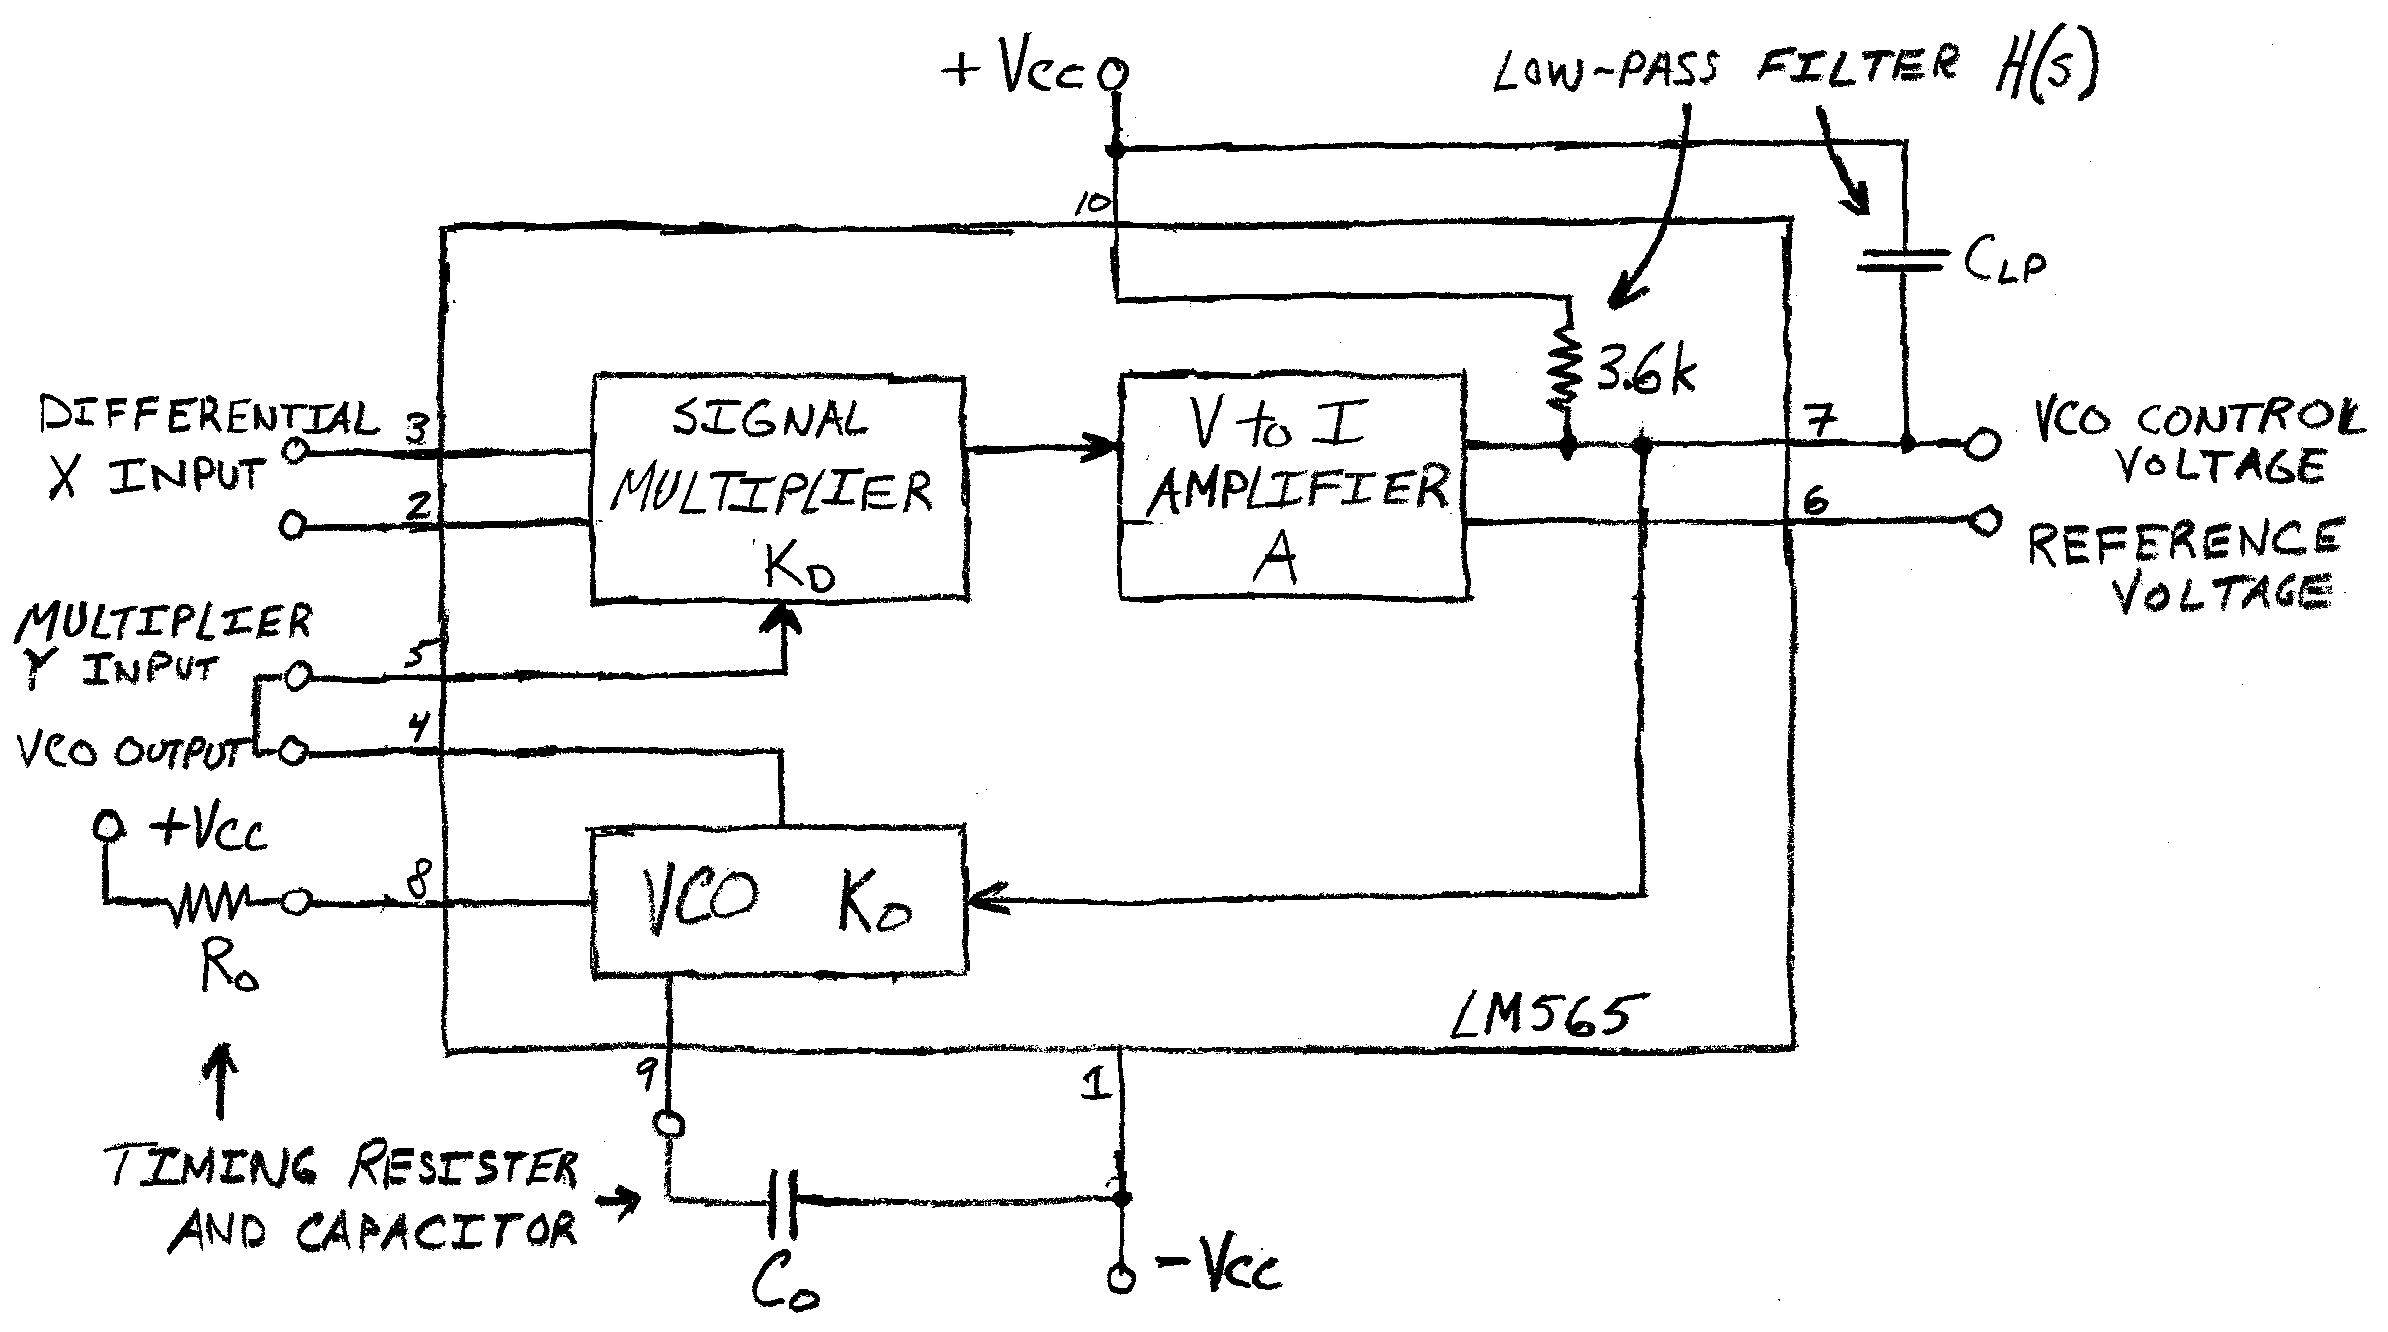
\includegraphics[width=0.75\textwidth]{diagrams/565-block-diagram}
	\caption{Rough Block Diagram for the LM565 Phase Locked Loop}
	\label{565-block-diagram}
\end{figure}

As discussed in the section \ref{principles-of-operation}, most of a PLL demodulator can be integrated onto a single silicon wafer--called a system-on-a-chip (SOC).
The only parts that cannot be fabricated on silicon are the capacitors, so the PLL demodulator has been redesigned with this in mind.
A company called Signetics was the first to put a PLL on an SOC, but they are out of business so we have a similar chip from Texas Instruments, the LM565.

The LM565 makes it easy for the circuit designer to incorporate frequency-shift keying into their product; you just have to slap on a few capacitors to have a working demodulator.
The only design that must be done is selecting a free-running frequency $f_{0}$ near the transmission frequency and building a low-pass filter with bandwidth greater than the frequency shift but less than twice the transmission frequency.
Use the following equation from the LM565 datasheet to select $f_{0}$.
\begin{equation}
f_{0}=\frac{0.3}{R_{0}C_{0}}
\label{f0-eq}
\end{equation}

For more information about how the LM565 works, see the schematic diagram in section \ref{lm565-schematic-diagram}.

\subsection{Voltage Controlled Oscillator}

\subsection{Signal Multiplier}

\subsection{Frequency Independent Amplifier}

\subsection{Low-Pass Filter}

\section{Design and Simulation}

\subsection{Voltage Controlled Oscillator}

\subsubsection{LM565 vs SPICE Model}

For the timing resistor $R_{0}$, I decided to use $3k\Omega$ because it was available with 1\% tolerance.
Using equation \ref{f0-eq}, the timing capacitors for 1 kHz, 10 kHz, and 100 kHz operating ranges should be
\begin{equation*}
R_{0}=3k\Omega
\end{equation*}
\begin{equation*}
C_{0(1kHz)}=0.1uF \quad | \quad C_{0(10kHz)}=0.01uF \quad | \quad C_{0(100kHz)}=1,000pF
\end{equation*}

\subsubsection{Free Running Frequency, $f_{0}$}

\subsubsection{Oscillator Sensitivity, $K_{O}$}

\subsection{Signal Multiplier}

\subsection{Frequency Independent Amplifier}

\subsection{Low-Pass Filter}

\subsection{Phase Detector Sensitivity, $K_{D}$}

\subsection{PLL Loop Gain, $K_{O}K_{D}$}

\subsection{FSK Generator}

\subsection{FSK Demodulator}

\section{Results}

\subsection{Free Running Frequency, $f_{0}$}

\subsection{Oscillator Sensitivity, $K_{O}$}

\subsection{FSK Demodulator}

\section{Conclusions}

\section{Appendices}

\clearpage
\subsection{LM565 Schematic Diagram}
\label{lm565-schematic-diagram}

\begin{figure}[ht]
	\centering
	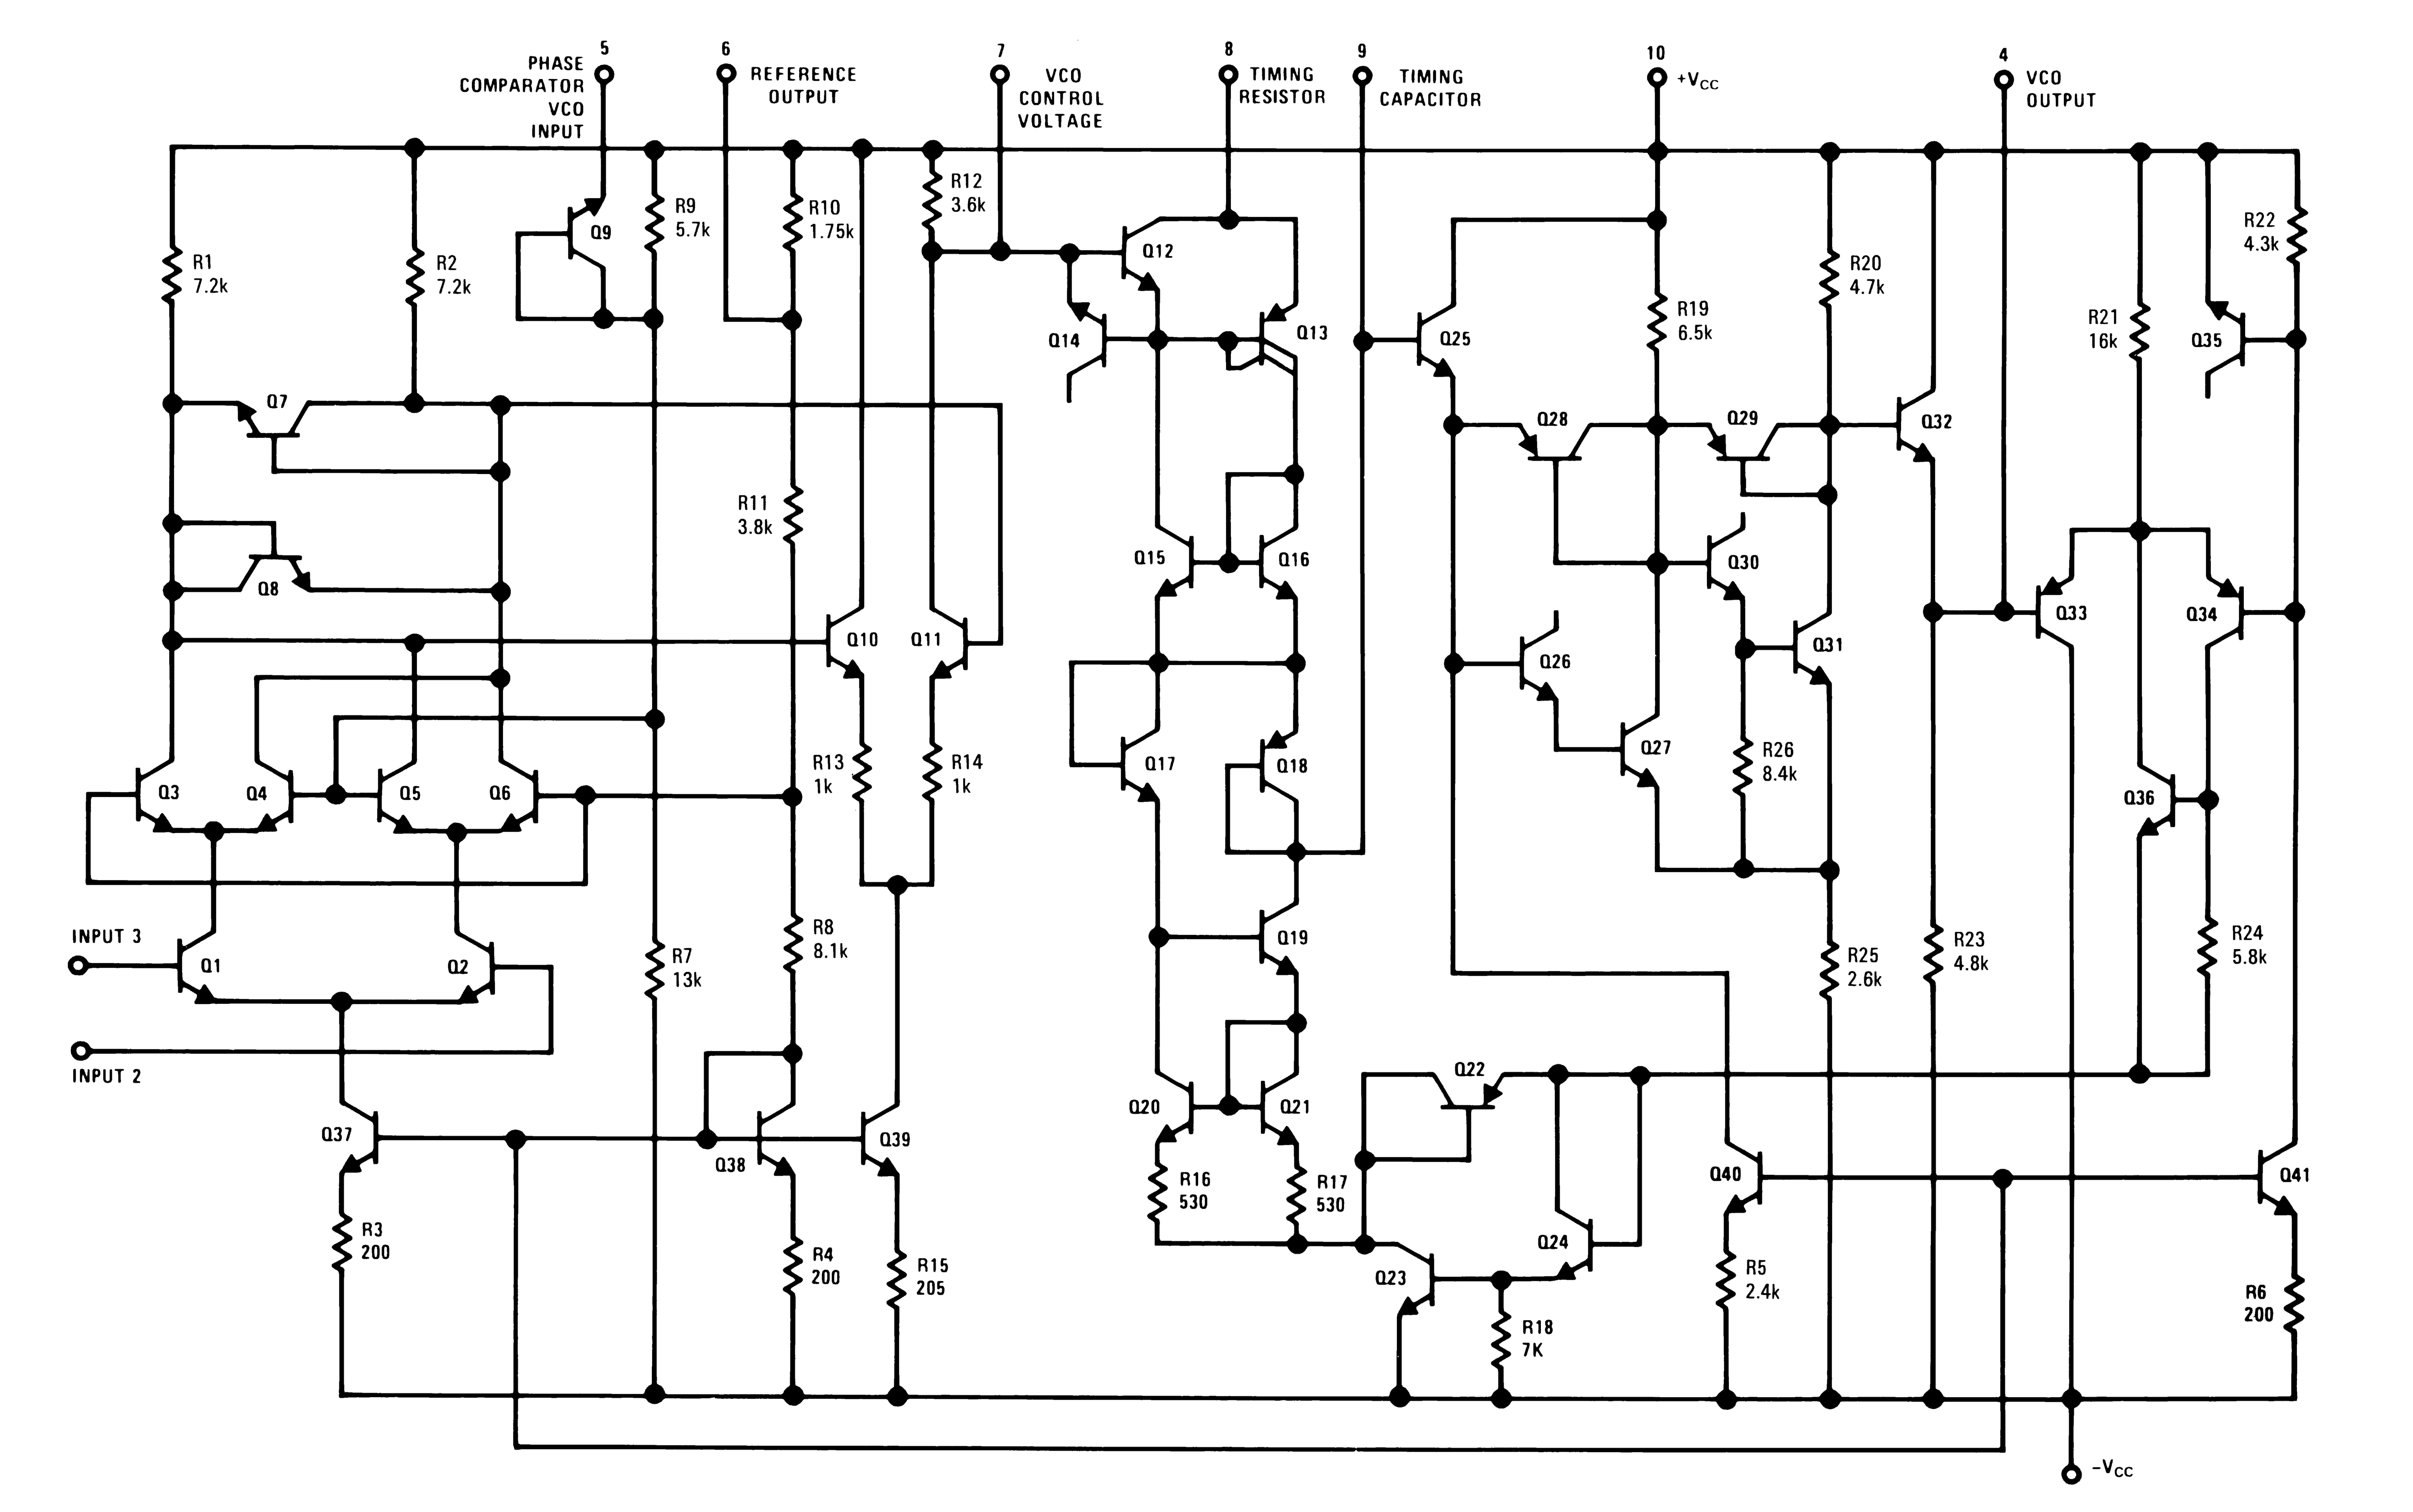
\includegraphics[width=1\textwidth]{diagrams/lm565-equivalent-circuit}
	\caption{LM565 Schematic Diagram; taken from page 6 of the TI datasheet}
	\label{lm565-equivalent-circuit}
\end{figure}

\end{document}
